%----------------------------------------------------------------------------------------
%	PACKAGES AND OTHER DOCUMENT CONFIGURATIONS
%----------------------------------------------------------------------------------------

\documentclass[final,hyperref={pdfpagelabels=false}]{beamer}

\usepackage[orientation=portrait,size=a0,scale=1.4]{beamerposter} % Use the beamerposter package for laying out the poster with a portrait orientation and an a0 paper size

\usetheme{I6pd2} % Use the I6pd2 theme supplied with this template
\usepackage[english]{babel} % English language/hyphenation
\usepackage{amsmath,amsthm,amssymb,latexsym} % For including math equations, theorems, symbols, etc

%\usepackage{times}\usefonttheme{professionalfonts}  % Uncomment to use Times as the main font
%\usefonttheme[onlymath]{serif} % Uncomment to use a Serif font within math environments

%\boldmath % Use bold for everything within the math environment

\graphicspath{{media/}} % Location of the graphics files
\usecaptiontemplate{\small\structure{\insertcaptionname~\insertcaptionnumber:\,}\insertcaption} % A fix for figure numbering
\usepackage{siunitx}

%set reference on one line
\setbeamertemplate{bibliography entry article}{}
\setbeamertemplate{bibliography entry title}{}
\setbeamertemplate{bibliography entry location}{}
\setbeamertemplate{bibliography entry note}{}

%----------------------------------------------------------------------------------------
%	TITLE SECTION 
%----------------------------------------------------------------------------------------

\title{\huge 3D Mapping of Glacier Moulins: Challenges and lessons learned} % Poster title

\author{\normalsize William Dubois,$^1$ Matěj Boxan,$^1$ Johann Laconte,$^2$ François Pomerleau$^1$} % Author(s)

\institute{\small$^1$ Northern Robotics Laboratory, Universit\'e Laval, Quebec City, Quebec, Canada \\ \small$^2$ French National Research Institute for Agriculture, Food and the Environment} % Institution(s)

%----------------------------------------------------------------------------------------
%	FOOTER TEXT
%----------------------------------------------------------------------------------------

\newcommand{\leftfoot}{IEEE International Conference on Robotics and Automation 2024} % Left footer text

\newcommand{\rightfoot}{william.dubois@norlab.ulaval.ca} % Right footer text

%----------------------------------------------------------------------------------------

\begin{document}

\addtobeamertemplate{block end}{}{\vspace*{1ex}} % White space under blocks

\begin{frame}[t] % The whole poster is enclosed in one beamer frame

\begin{columns}[t] % The whole poster consists of two major columns, each of which can be subdivided further with another \begin{columns} block - the [t] argument aligns each column's content to the top

\begin{column}{.02\textwidth}\end{column} % Empty spacer column

\begin{column}{.465\textwidth} % The first column

%----------------------------------------------------------------------------------------
%	OBJECTIVES
%----------------------------------------------------------------------------------------

\begin{block}{Context \& Motivations}
\begin{itemize}
	\item Deploying robots in the cryosphere is still an open problem \cite{Pomerleau2023}, and is a crucial source of data collection and analysis, essential for understanding problems such as climate change.
	\item Dante was the first robot successfully deployed in a remote hazardous setting, an Alaskan volcano \cite{Dante2}, demonstrating feasibility 
	\item Prior deployments have shown the hazardous conditions surrounding surveys within glaciers \cite{Talbot2023, Polzin2023} and have highlighted the potential of robotic platforms in monitoring changes.
\end{itemize}
\end{block}

\begin{block}{Experimental platform}
	\begin{itemize}
		\item We designed and developed a measurement platform capable of sustaining significant forces caused by various extreme motions and collisions that can occur in extreme environments.
		\item The platform is built to record data from sensors needed to perform localization and mapping using a Raspberry Pi 4B.
		\item Data is then post-processed to complete the localization and mapping and evaluate its performances.
		\item To ensure no pollution is left on-site if anything breaks, a safety net was installed on the platform, thin enough not to cause any occlusions.
	\end{itemize}
	\centering
	\begin{figure}
		\includegraphics[width=0.95\linewidth]{figures/robot.pdf}
		\caption{Data gathering platform with which sensor measurements were recorded to perform 3D localization and mapping, equipped with a lidar Robosense RS-16 (\texttt{1}), an Xsens MTi-10 IMU (\texttt{2}), a Vectornav vn100 IMU (\texttt{3}, behind the Xsens MTi-10) and a barometric pressure sensor DPS310 (\texttt{4}, on the other side of the platform).}
	\end{figure}
\end{block}

\begin{block}{Experiments}
	\begin{columns} % Subdivide the first main column
		\begin{column}{.5\textwidth} % The first subdivided column within the first main column
			\centering
			\begin{figure}
				\vspace{-25mm}
				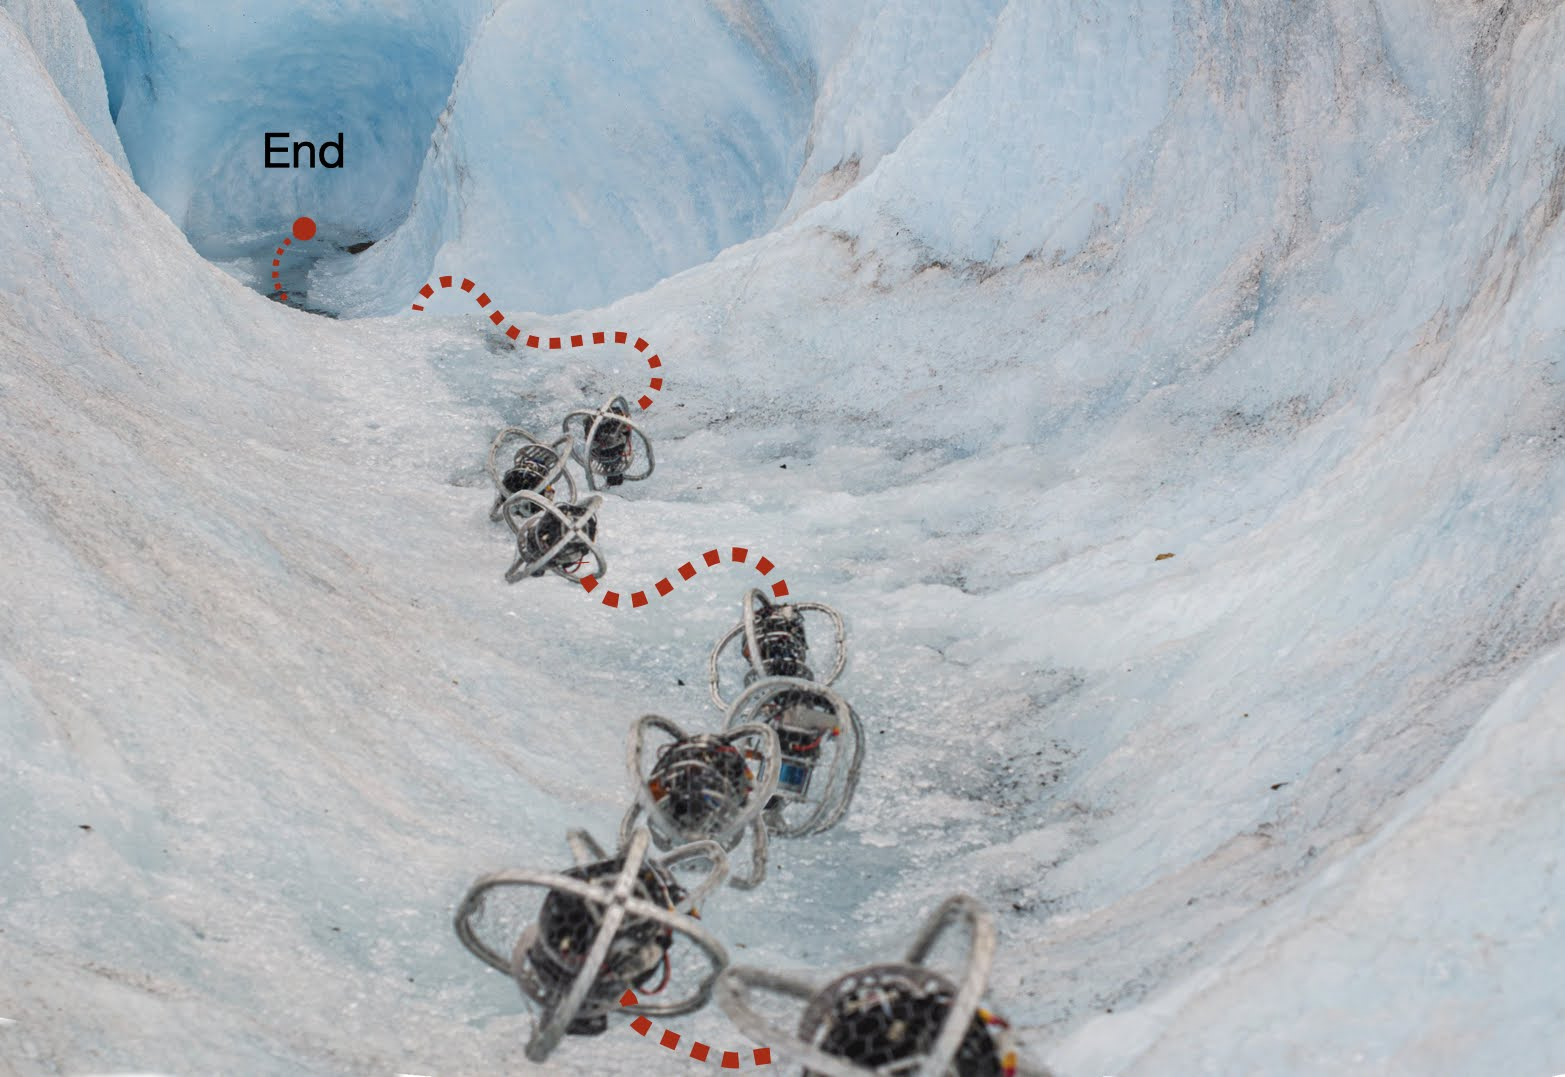
\includegraphics[width=0.95\linewidth]{figures/ice_canyon.jpeg}
				\caption{The experimental platform rolled down a \SI{30}{\meter} ice canyon.}
			\end{figure}
			\begin{itemize}
				\item \textbf{Glacial moulin}: 
				\begin{itemize}
					\item Low feature environment.
					\item The platform is initially lowered down the moulin while recording sensor measurements.
					\item Ultimately, the platform was thrown in the moulin to record measurements through extreme motions such as free fall.
				\end{itemize}
			\end{itemize}
		\end{column}
		\begin{column}{.5\textwidth} % The second subdivided column within the first main column
			\begin{itemize}
				\item \textbf{Ice canyon}: 
				\begin{itemize}
					\item Low difficulty experiment.
					\item The platform rolled down an ice canyon while recording sensor measurements.
					\item Environment with enough constraints and easy access to quickly validate the impact of ice and various factors on the platform.
				\end{itemize}
			\end{itemize}
			\centering
			\begin{figure}
				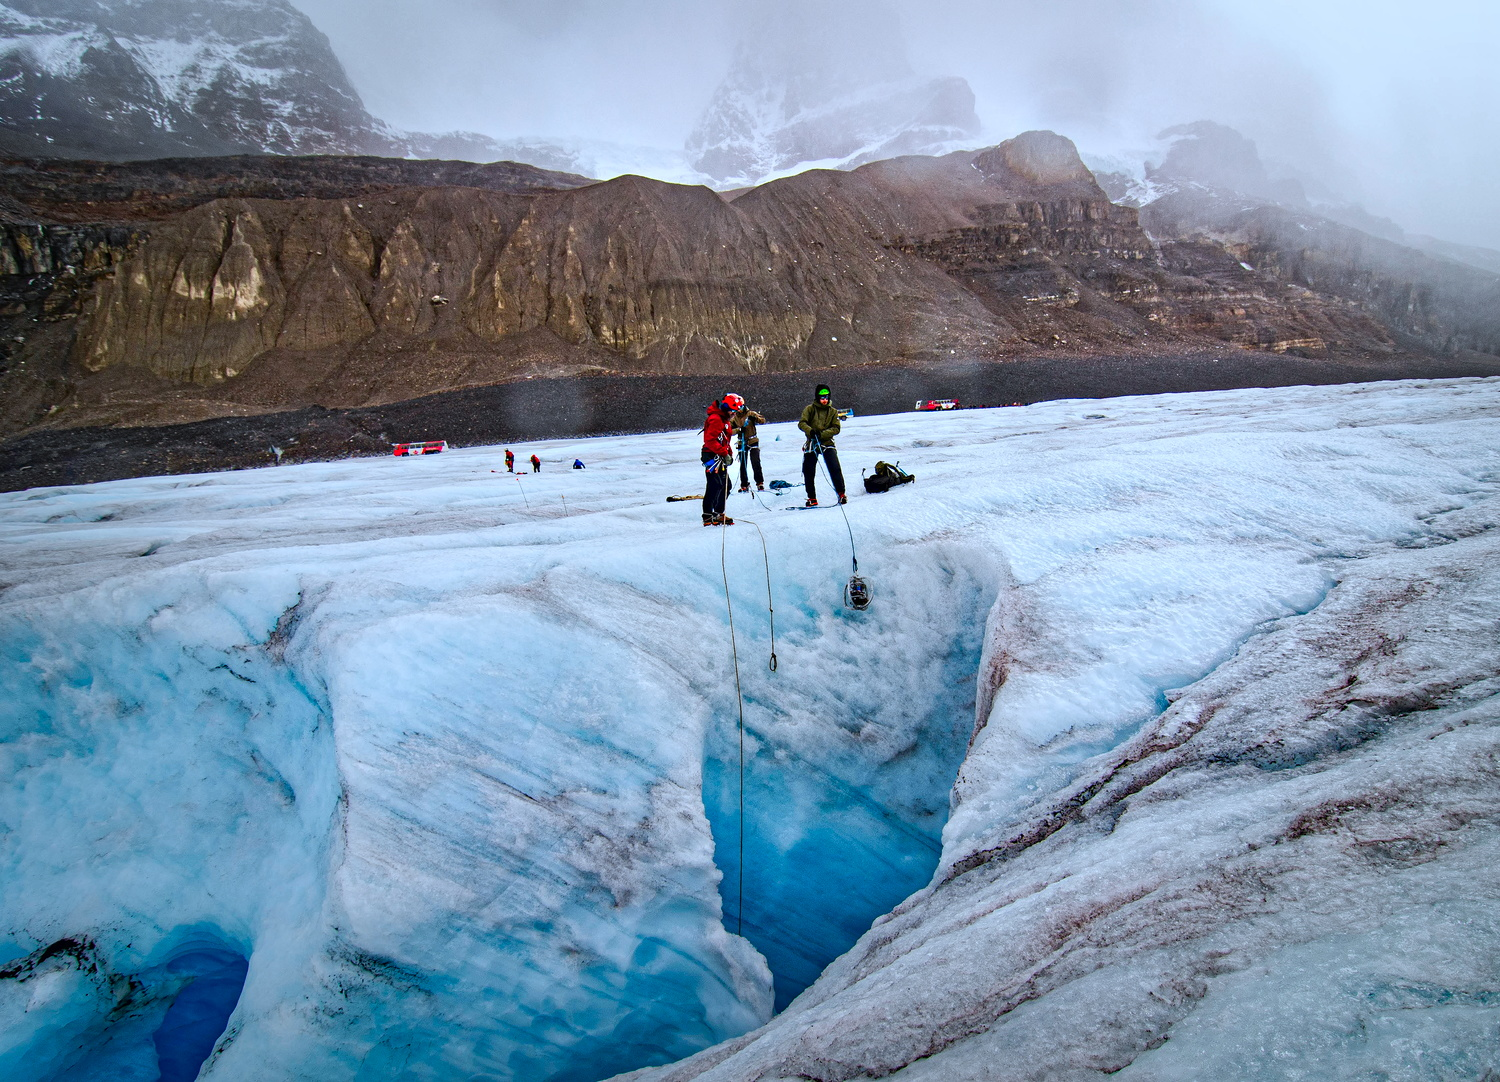
\includegraphics[width=0.95\linewidth]{figures/sphere_moulin_improved_small.jpg}
				\caption{The experimental platform was lowered in a glacial moulin, mapping its surroundings.}
			\end{figure}
		\end{column}
	\end{columns} % End of the subdivision
\end{block}

%----------------------------------------------------------------------------------------

\end{column} % End of the first column

\begin{column}{.03\textwidth}\end{column} % Empty spacer column
 
\begin{column}{.465\textwidth} % The second column
	
%----------------------------------------------------------------------------------------
%	New block	
%----------------------------------------------------------------------------------------

\begin{block}{Challenges and lessons learned}
	\begin{itemize}
		\item \textbf{Extreme environments} lead to:
		\begin{itemize}
			\item erratic weather conditions necessitating rugged equipment and dedicated specialized equipments,
			\item stringent safety measures and extreme conditions that add additional stress on your body and mind.
		\end{itemize}
		\item \textbf{Preparation} is key:
		\begin{itemize}
			\item thorough and tested experimental and validation procedure are necessary,
			\item spare equipment is crucial, everything that can break will break.
		\end{itemize}
	\end{itemize}
\end{block}

%----------------------------------------------------------------------------------------
%	New block
%----------------------------------------------------------------------------------------

\begin{block}{Results}
\begin{itemize}
	\item Lidar and IMU measurements enabled us to compute 3D mapping and localization of the experimental platform throughout its slow descent in the moulin.
	\item Experiments were conclusive, but only low quality maps were obtainable. 
\end{itemize}
\begin{figure}
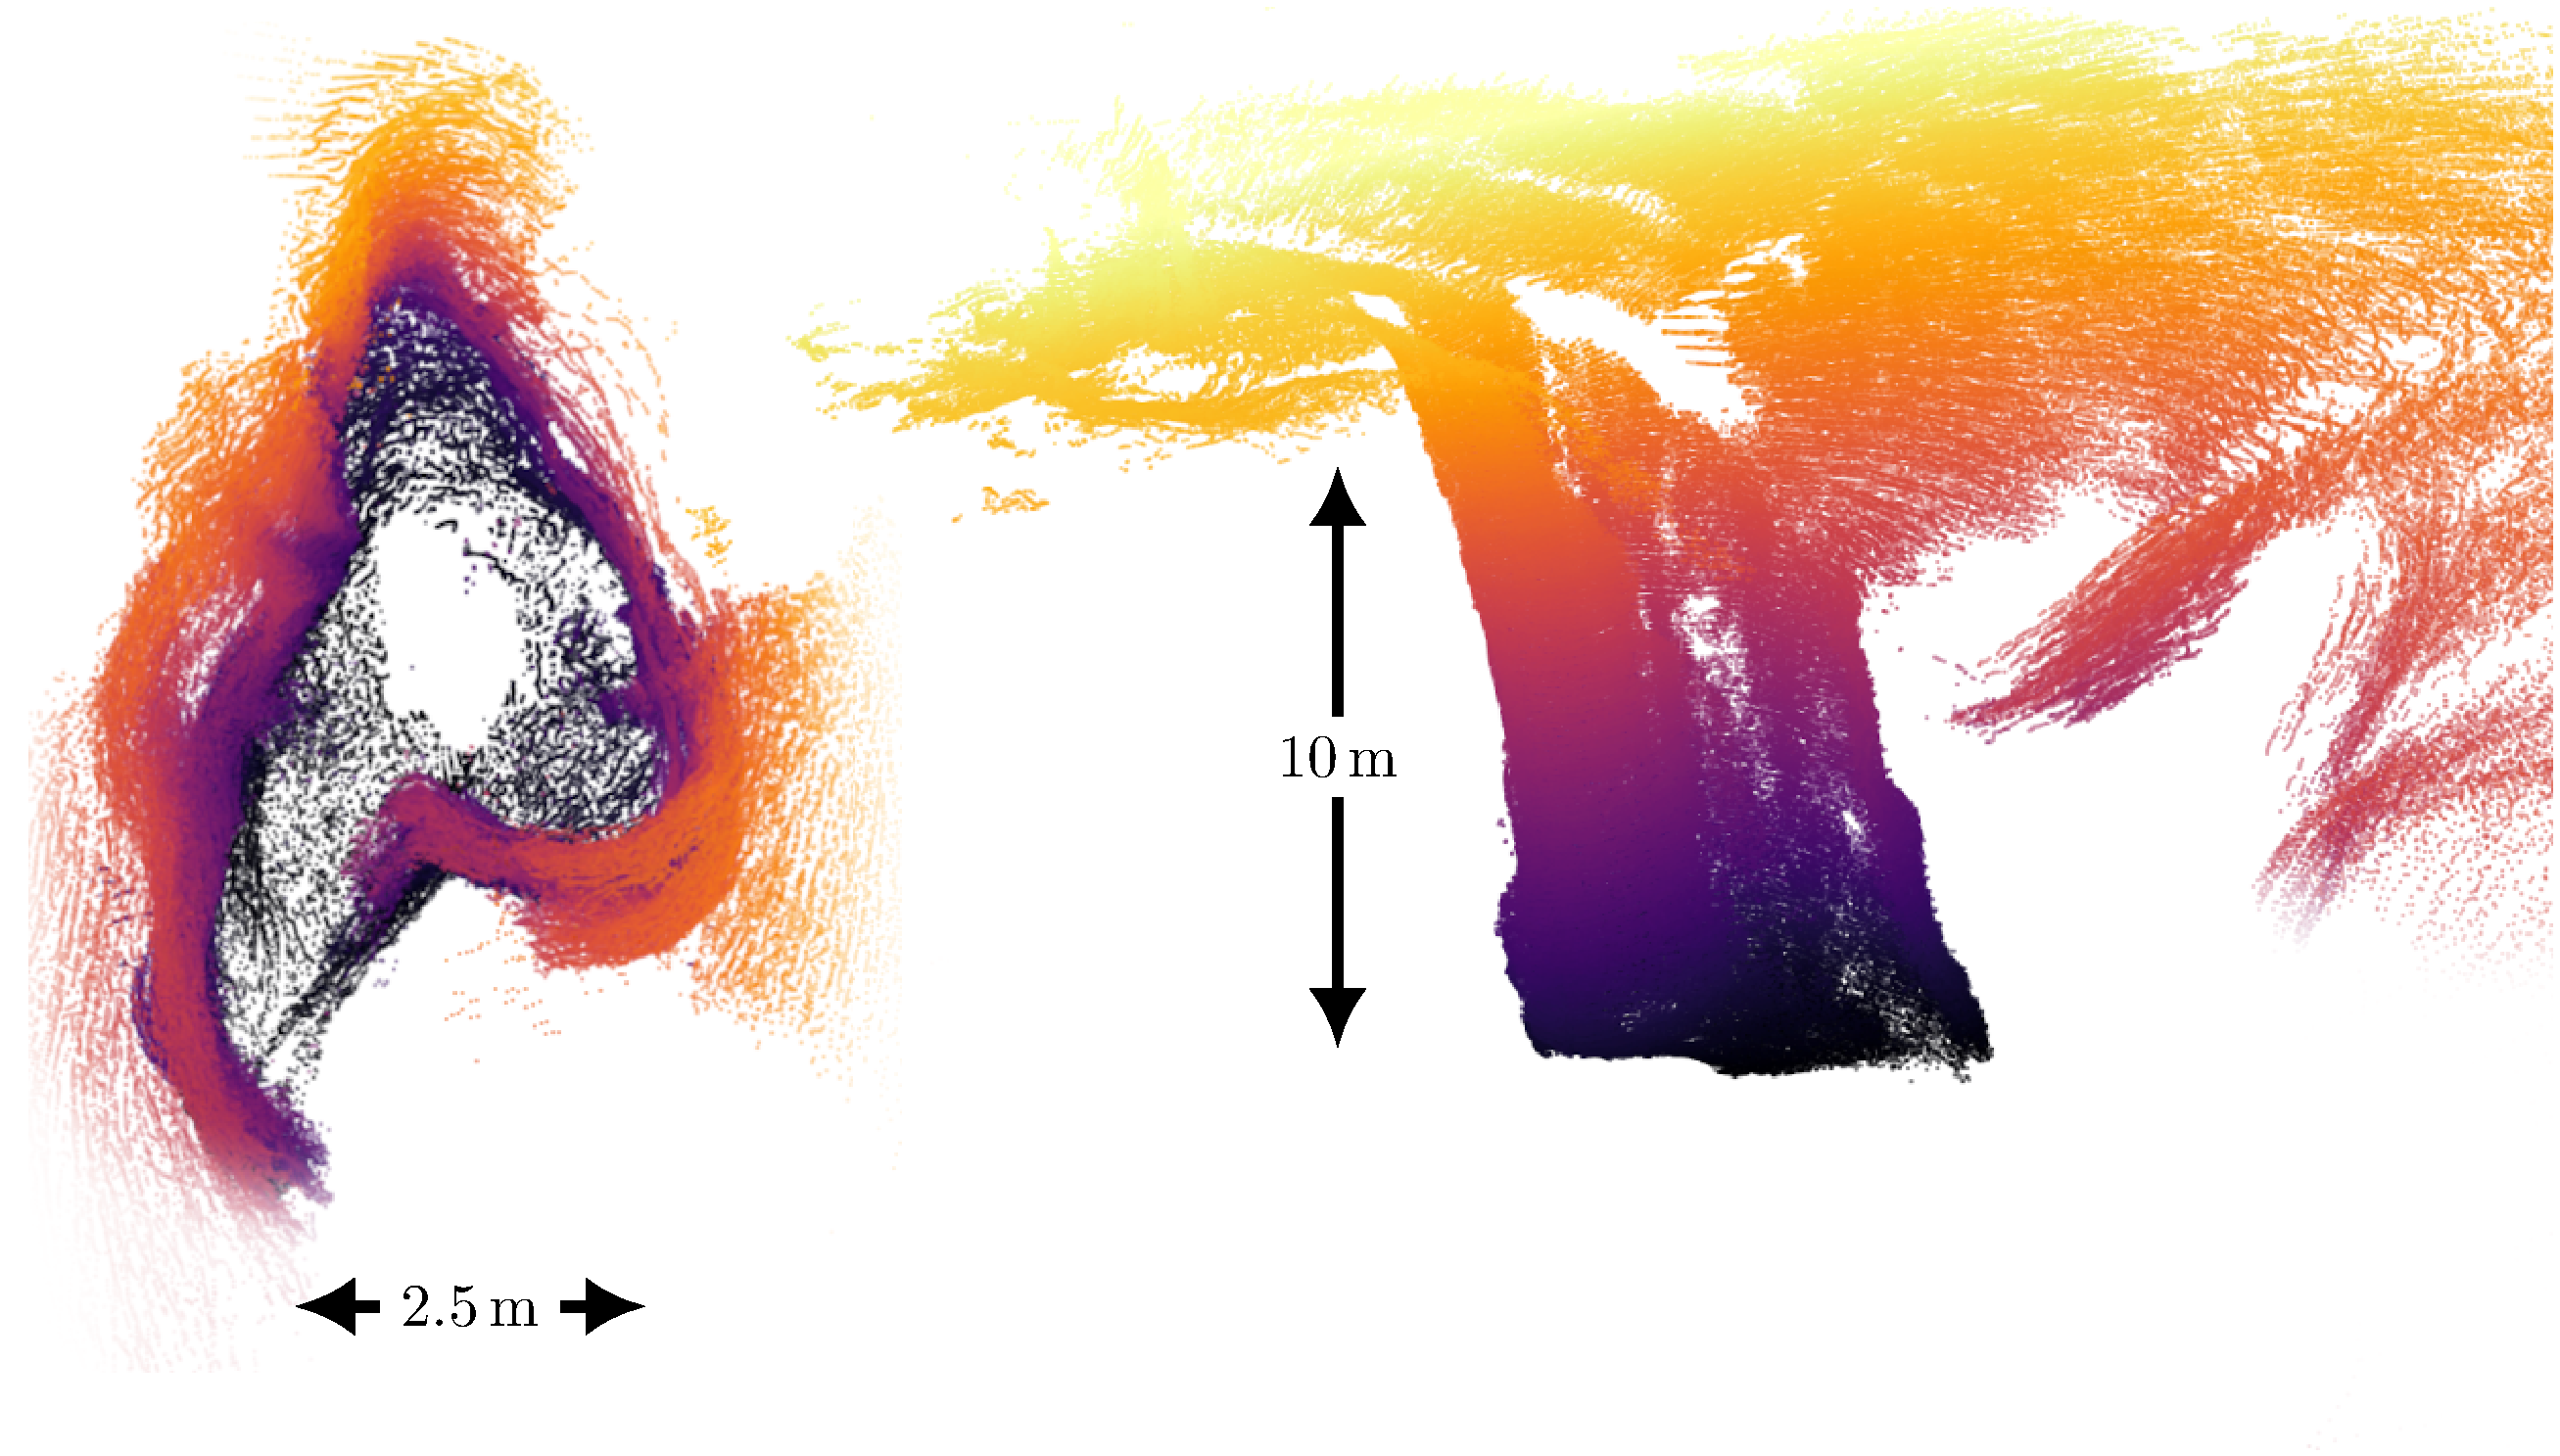
\includegraphics[width=1.0\linewidth]{figures/moulin2.pdf}%
\vspace{-7mm}
\caption{Map result (colored by elevation) from the moulin experiment. Left: top view; Right: Side view. The lack of features in the moulin makes the mapping of such environments challenging.}
\label{fig:3D-map}
\end{figure}
\begin{itemize}
	\item Lack of features led to: 
	\begin{itemize}
		\item under-constrained and degraded registration solutions,
		\item lower quality maps,
		\item lower quality information about the surveyed environment.
	\end{itemize}
	\item Addition of barometric pressure information can help gain constraints.
\end{itemize}
\end{block}

%----------------------------------------------------------------------------------------
%	New block	
%----------------------------------------------------------------------------------------

\begin{block}{Future works}
	\begin{itemize}
		\item \textbf{Increase mapping performances and robustness} through fusion of information from several sensors, including atmospheric pressure.
		\item \textbf{Improvement of the experimental platform} to increase its robustness and versatility. 
	\end{itemize}
\end{block}

%----------------------------------------------------------------------------------------
%	ACKNOWLEDGEMENTS
%----------------------------------------------------------------------------------------

\begin{block}{Acknowledgments and References}
\footnotesize%
\noindent This research was supported by the Natural Sciences and Engineering Research Council of Canada (NSERC) through the General Research Fund (GRF) from Universit\'e Laval.
\nocite{*} % Insert publications even if they are not cited in the poster
\bibliographystyle{unsrt}%
{\footnotesize\bibliography{biblio}}
\vspace{-3mm}
\end{block}

%----------------------------------------------------------------------------------------
%	CONTACT INFORMATION
%----------------------------------------------------------------------------------------
%
%\setbeamercolor{block title}{fg=black,bg=orange!70} % Change the block title color
%
%\begin{block}{Contact Information}
%
%\begin{itemize}
%\item Web: \href{http://www.university.edu/smithlab}{http://www.university.edu/smithlab}
%\item Email: \href{mailto:john@smith.com}{john@smith.com}
%\item Phone: +1 (000) 111 1111
%\end{itemize}
%
%\end{block}

%----------------------------------------------------------------------------------------

\end{column} % End of the second column

\begin{column}{.015\textwidth}\end{column} % Empty spacer column
\end{columns} % End of all the columns in the poster
%----------------------------------------------------------------------------------------
%	REFERENCES
%----------------------------------------------------------------------------------------
%
%\begin{block}{Acknowledgments and References}
%	\small
%	\noindent This research was supported by the Natural Sciences and Engineering Research Council of Canada (NSERC) through the General Research Fund (GRF) from Université Laval.
%	\nocite{*} % Insert publications even if they are not cited in the poster
%	\bibliographystyle{unsrt}%
%	{\small\bibliography{biblio}}
%	\vspace{-3mm}
%\end{block}

\end{frame} % End of the enclosing frame

\end{document}
